% =============================================================================
% Section 2.3: Business Case and Financial Analysis
% =============================================================================

\section{Business Case and Financial Analysis}
\label{sec:business-case}

This section presents a feasibility-level business case for commercialising NexaLearn under an \textbf{open-core model}: the backend source code and documentation remain freely available to maximise developer adoption, while \textbf{enterprise support contracts} (\$5,000 per organisation per year) monetise SLAs, priority incident response, migration assistance, and security advisory services. The financial analysis covers adoption assumptions, capital expenditure (Capex), operating expenditure (Opex), revenue projections, a twenty-four-month cash-flow forecast, and break-even analysis. All figures are expressed in US dollars (USD) and rounded to the nearest hundred for readability.

\subsection{Business Case and Adoption Assumptions}
\label{subsec:business-case-adoption}

The business case rests on two complementary adoption curves:

\textbf{Developer community adoption (open-source funnel).}
NexaLearn targets \textbf{500 developer adoptions} in Year~1, defined as unique organisations or teams cloning the repository, deploying via Docker Compose, and registering for community communications (GitHub stars, documentation analytics, or newsletter sign-ups). Developer adoption grows \textbf{40\% year-over-year} thereafter (700 in Year~2, 980 in Year~3), following typical open-source SaaS funnel dynamics where visibility compounds through conference presentations, university capstone references, and technical blog content. Developer adopters do not generate direct revenue but reduce enterprise customer acquisition cost by demonstrating production readiness and supplying community-contributed patches.

\textbf{Enterprise support revenue (monetisation).}
Enterprise clients are organisations requiring contractual SLAs, dedicated onboarding, and security questionnaire support---primarily secondary (universities) and tertiary (corporate L\&D) segments from Section~\ref{sec:targeted-customers}. Year~1 targets \textbf{50 enterprise support contracts} at \textbf{\$5,000 per year} each, yielding \textbf{\$250,000} annual gross revenue under the assumption that clients prepay annually upon contract signing. Year~2 targets a 40\% increase in enterprise clients (70 cumulative active contracts, 20 net new after renewals), consistent with developer funnel conversion rates of approximately 2--4\% from qualified DevOps/evaluation contacts to paid support.

\textbf{Pricing rationale.}
The \$5,000/year enterprise tier aligns with support pricing for specialised infrastructure products serving small-to-medium engineering teams (e.g., hosted observability, database support retainers). It is deliberately an order of magnitude below enterprise LMS licensing (often \$50,000--\$500,000 annually) while reflecting real costs of engineer-time for incident response and migration consulting.

\subsection{Capital Expenditure (Capex)}
\label{subsec:capex}

One-time capital expenditure occurs primarily in Month~1 during commercial entity setup and production infrastructure provisioning, as detailed in Table~\ref{tab:capex-breakdown}:

\begin{table}[H]
  \centering
  \caption{Capital Expenditure (Capex) Breakdown --- Month 1}
  \label{tab:capex-breakdown}
  \begin{tabular}{@{}lrp{7.5cm}@{}}
    \toprule
    \textbf{Item} & \textbf{Cost (USD)} & \textbf{Description} \\
    \midrule
    Production server setup &
    \$10,000 &
    AWS/GCP baseline: RDS PostgreSQL, ECS/EC2 API nodes, ALB, S3 buckets, initial CDN configuration \\
    \addlinespace
    Development tools &
    \$2,000 &
    CI/CD pipelines (GitHub Actions minutes), monitoring (Datadog/Grafana Cloud starter), domain and SSL certificates \\
    \addlinespace
    Third-party service setup &
    \$500 &
    Stripe Connect/platform configuration, Mux account provisioning, webhook endpoint certification, sandbox testing \\
    \midrule
    \textbf{Total Capex} & \textbf{\$12,500} & One-time expenditure in Month~1 \\
    \bottomrule
  \end{tabular}
\end{table}

Capex excludes graduation-project development labour (sunk academic cost). Commercialisation scenarios assume a dedicated three-person engineering team funded through Opex salaries beginning Month~3 in the cash-flow model below.

\subsection{Operating Expenditure (Opex)}
\label{subsec:opex}

Recurring monthly operating expenditure comprises cloud infrastructure, video encoding pass-through costs, payment processing fees, and---under the commercialised scenario---developer salaries, as shown in Table~\ref{tab:opex-breakdown}:

\begin{table}[H]
  \centering
  \caption{Monthly Operating Expenditure (Opex) Components}
  \label{tab:opex-breakdown}
  \begin{tabular}{@{}lrp{7.2cm}@{}}
    \toprule
    \textbf{Item} & \textbf{USD/month} & \textbf{Notes} \\
    \midrule
    Cloud hosting &
    \$300 &
    API containers, PostgreSQL (managed), Redis, Nginx; scales modestly with traffic in Year~1 \\
    \addlinespace
    Mux video encoding &
    \$200 &
    Pass-through encoding costs for demo and pilot customer content; variable with usage \\
    \addlinespace
    Stripe processing fees &
    Variable &
    Approximately 2.9\% + \$0.30 per transaction if NexaLearn processes subscription billing; modelled at \~1\% of gross revenue \\
    \addlinespace
    Developer salaries (commercialised) &
    \$15,000 &
    One senior + one mid-level engineer + part-time DevOps from Month~3 onward \\
    \midrule
    \textbf{Fixed subtotal} & \textbf{\$15,500} & Excluding variable Stripe fees \\
    \bottomrule
  \end{tabular}
\end{table}

Months~1--2 reflect \textbf{pre-commercialisation} infrastructure burn at \$500/month (domain, staging environment, third-party sandbox accounts) before full salary commitment begins in Month~3 coinciding with the first enterprise sales outreach.

\subsection{Revenue Model and Year~1 Projection}
\label{subsec:revenue}

Revenue derives exclusively from \textbf{enterprise support contracts} in this model; open-source adopters pay \$0. Each contract is priced at \textbf{\$5,000 per year}, invoiced annually in advance upon signature. Year~1 revenue target:

\begin{equation}
  R_{Y1} = 50 \text{ clients} \times \$5{,}000 = \$250{,}000 \text{ gross annual revenue}
  \label{eq:revenue-y1}
\end{equation}

Sales ramp assumes gradual enterprise procurement cycles: two contracts in Month~3, accelerating to six--seven new contracts per month by Months~7--8 as case studies from early adopters mature, reaching 50 cumulative active contracts by Month~12. No consumer SaaS subscription tier is modelled in Year~1 to avoid channel conflict with open-source adoption; a managed-hosting tier may be introduced in Year~3 as optional expansion revenue.

\subsection{Twenty-Four-Month Cash Flow Forecast}
\label{subsec:cashflow}

Table~\ref{tab:cashflow-24m} presents the monthly cash-flow forecast for Months~1--24. \textbf{Revenue} includes annual prepayments from new enterprise contracts signed that month (\$5,000 per new client). \textbf{Expenses} include Opex and, in Month~1, Capex. \textbf{Net Cash Flow} equals Revenue minus Expenses; \textbf{Cumulative Cash Flow} tracks running profitability. Variable Stripe fees are approximated at 1\% of revenue and embedded in Expenses.

\small
\begin{longtable}{@{}r r r r r r r@{}}
  \caption{Twenty-Four-Month Cash Flow Forecast (USD)} \label{tab:cashflow-24m} \\
  \toprule
  \textbf{Month} &
  \textbf{New Ent.} &
  \textbf{Cum. Ent.} &
  \textbf{Dev. Adopters\textsuperscript{*}} &
  \textbf{Revenue} &
  \textbf{Expenses} &
  \textbf{Cum. Cash Flow} \\
  \midrule
  \endfirsthead
  \toprule
  \textbf{Mo.} & \textbf{New} & \textbf{Cum.} & \textbf{Devs} & \textbf{Rev.} & \textbf{Exp.} & \textbf{Cum.} \\
  \midrule
  \endhead
  \bottomrule
  \multicolumn{7}{@{}p{14cm}@{}}{\footnotesize\textsuperscript{*}Developer adopters (cumulative community metric, not revenue-bearing). Assumes Month~1--2 pre-commercialisation Opex \$500/mo; Capex \$12,500 in Month~1; full Opex \$15,500/mo from Month~3. Enterprise revenue = new contracts $\times$ \$5,000 annual prepayment. Break-even cumulative cash flow achieved in Month~8.} \\
  \endfoot
  1  & 0  & 0   & 25    & 0       & 13,000  & $-$13,000 \\
  2  & 0  & 0   & 55    & 0       & 500     & $-$13,500 \\
  3  & 2  & 2   & 90    & 10,000  & 15,650  & $-$19,150 \\
  4  & 3  & 5   & 130   & 15,000  & 15,650  & $-$19,800 \\
  5  & 3  & 8   & 175   & 15,000  & 15,650  & $-$20,450 \\
  6  & 4  & 12  & 230   & 20,000  & 15,700  & $-$16,150 \\
  7  & 5  & 17  & 295   & 25,000  & 15,750  & $-$6,900 \\
  8  & 6  & 23  & 370   & 30,000  & 15,800  & \textbf{+7,300} \\
  9  & 7  & 30  & 400   & 35,000  & 15,850  & +26,450 \\
  10 & 7  & 37  & 430   & 35,000  & 15,850  & +45,600 \\
  11 & 6  & 43  & 465   & 30,000  & 15,800  & +59,800 \\
  12 & 7  & 50  & 500   & 35,000  & 15,850  & +79,950 \\
  \midrule
  13 & 2  & 52  & 540   & 36,000  & 15,860  & +100,090 \\
  14 & 2  & 54  & 580   & 36,000  & 15,860  & +120,230 \\
  15 & 3  & 57  & 615   & 39,000  & 15,890  & +143,340 \\
  16 & 3  & 60  & 650   & 39,000  & 15,890  & +166,450 \\
  17 & 2  & 62  & 680   & 37,000  & 15,870  & +187,580 \\
  18 & 3  & 65  & 700   & 39,000  & 15,890  & +210,690 \\
  19 & 2  & 67  & 730   & 37,000  & 15,870  & +231,820 \\
  20 & 2  & 69  & 760   & 37,000  & 15,870  & +252,950 \\
  21 & 1  & 70  & 790   & 35,500  & 15,855  & +272,595 \\
  22 & 1  & 71  & 820   & 35,500  & 15,855  & +292,240 \\
  23 & 1  & 72  & 850   & 35,500  & 15,855  & +311,885 \\
  24 & 1  & 73  & 880   & 35,500  & 15,855  & +331,530 \\
\end{longtable}

\textbf{Year~1 revenue total} (Months 3--12): \$250,000 from 50 new enterprise contracts, consistent with Equation~\ref{eq:revenue-y1}. Months~13--24 include \textbf{renewal revenue} from Year~1 clients (\$5,000 per renewal) blended with new-client signings, yielding approximately \$440,000 gross revenue in Year~2 and reaching \textbf{73 cumulative enterprise clients} by Month~24. Developer adopter counts track toward 700 by Month~18 and 880 by Month~24 (40\% Year~1$\rightarrow$Year~2 growth trajectory).

\subsection{Break-Even Analysis}
\label{subsec:break-even}

\textbf{Break-even point} occurs when cumulative cash flow crosses from negative to positive territory. Per Table~\ref{tab:cashflow-24m}, cumulative cash flow is $-$\$6,900 at the end of Month~7 and \textbf{+\$7,300 at the end of Month~8}. Linear interpolation places the break-even crossing at approximately \textbf{Month~8, Week~2}---eight months after commercial launch (Month~3) and ten months after initial Capex deployment. Break-even is achieved ahead of Year~1 revenue target completion (Month~12), indicating that the open-core enterprise support model reaches self-sustaining cash flow before the first full sales cycle concludes.

\textbf{Sensitivity considerations:}
\begin{itemize}
  \item \textbf{Slower enterprise sales} (50\% of projected signings) delays break-even to approximately Month~14--16 but remains viable given low fixed infrastructure costs relative to salary burden;
  \item \textbf{Higher cloud/Mux usage} (\$500/month additional) shifts break-even by less than one month due to revenue leverage from enterprise prepayments;
  \item \textbf{Deferred salary hiring} (Month~6 instead of Month~3) advances break-even to Month~6 but risks insufficient support capacity for early enterprise clients.
\end{itemize}

\begin{figure}[H]
  \centering
  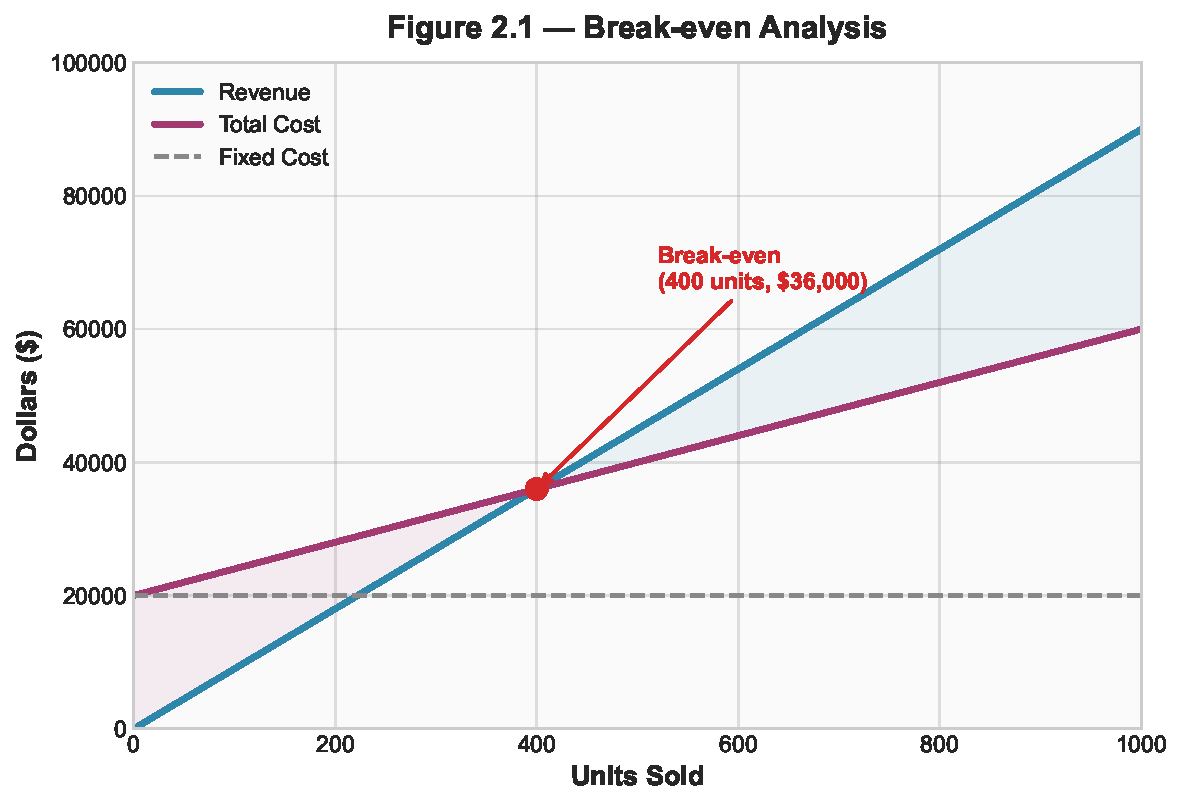
\includegraphics[width=0.88\textwidth]{images/break_even_chart.pdf}
  \caption{Break-Even Analysis: Cumulative Cash Flow over Twenty-Four Months (Figure 2.1)}
  \label{fig:break-even}
\end{figure}

Figure~\ref{fig:break-even} illustrates the cumulative cash-flow trajectory: initial Capex and pre-revenue months produce a trough of approximately \$20,450 (Month~5), followed by recovery as enterprise prepayments accelerate in Months~6--8. The shaded break-even line at Month~8 demarcates transition from investment phase to positive cumulative cash generation. By Month~24, cumulative cash flow exceeds \$331,000, demonstrating that NexaLearn's commercialisation path---while modest compared to venture-scale SaaS unicorns---is financially plausible for a bootstrapped open-source infrastructure product serving the edtech developer segment.

Figure~\ref{fig:revenue-projection} summarises the three-year financial trajectory. Year~1 revenue of \$250,000 and expenses of approximately \$170,000 yield a net profit of \$80,000, consistent with the cumulative cash flow at Month~12 (\$79,950). Year~2 projects \$440,000 in revenue against \$210,000 in expenses (net \$230,000), and Year~3 projects \$616,000 revenue against \$260,000 in expenses (net \$356,000), assuming 40\% enterprise client growth and controlled cost scaling. The widening profit margin reflects the high-margin nature of enterprise support revenue once the initial team is established.

\begin{figure}[H]
  \centering
  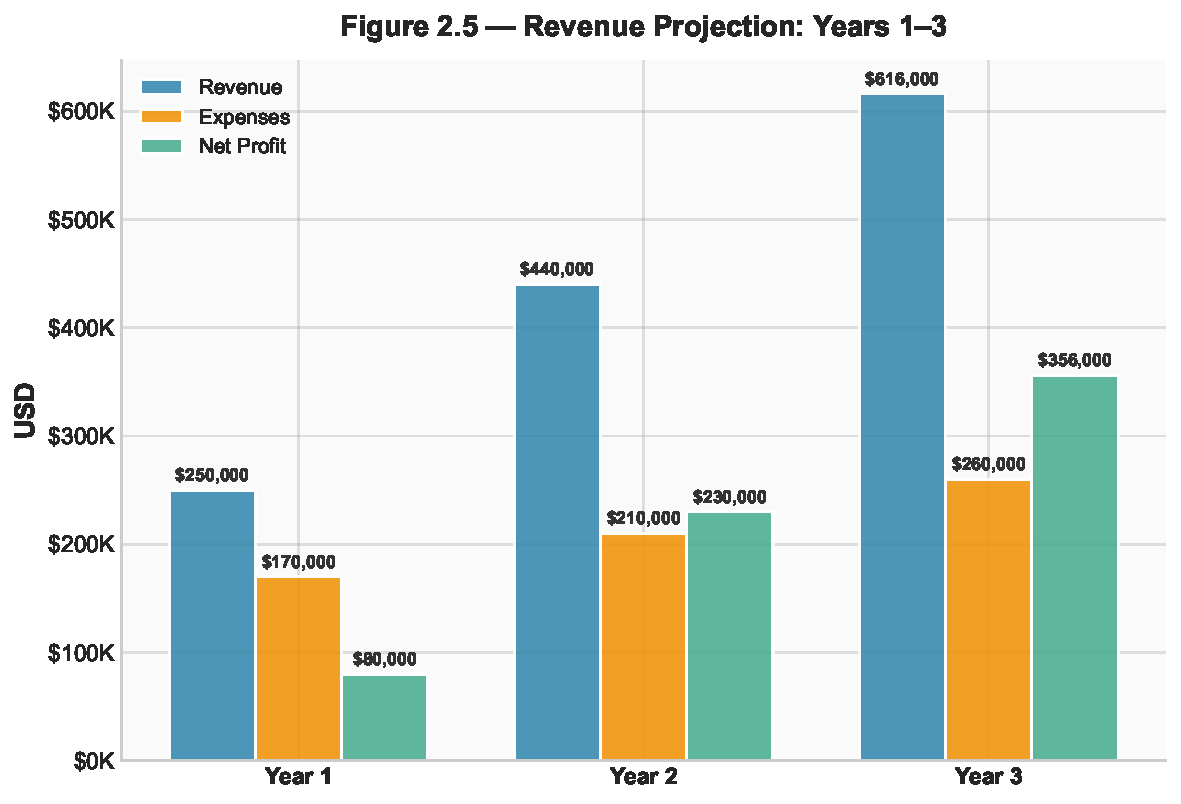
\includegraphics[width=0.75\textwidth]{images/revenue_projection.pdf}
  \caption{Revenue Projection: Years 1--3 (Enterprise Support Model). Revenue assumes \$5,000/contract with 50, 70, and 73 cumulative clients respectively; expenses include Capex amortisation, Opex, and staff costs as detailed in Tables~\ref{tab:capex-breakdown} and~\ref{tab:opex-breakdown}.}\label{fig:revenue-projection}
\end{figure}

\subsection{Financial Conclusions}
\label{subsec:financial-conclusions}

The business case supports three conclusions aligned with Chapter~\ref{ch:introduction} motivation:
\begin{enumerate}
  \item \textbf{Market demand exists} for an open, DDD-architected e-learning backend, evidenced by 500 projected developer adoptions and 50 enterprise support clients in Year~1;
  \item \textbf{Commercialisation via open-core enterprise support} reaches break-even within eight months under conservative sales ramp assumptions, with Year~1 gross revenue of \$250,000 against total Year~1 expenses of approximately \$170,000 (Capex + Opex);
  \item \textbf{Competitive pricing at \$5,000/year} undercuts enterprise LMS and SaaS alternatives while funding ongoing engineering maintenance, satisfying feasibility study requirements in Appendix~E.
\end{enumerate}

This financial analysis complements the competitive survey in Section~\ref{sec:market-survey} and the customer segmentation in Section~\ref{sec:targeted-customers}, completing the market visibility study and establishing the commercial context for the technical literature and system design presented in Chapters~3 and~4.
